\chapter{Models and Simulations}
\label{chapter:mods-sims}
	%Most of the general details are presented before the first section.
	
	%Broad/non-focused introduction to section.
	A simulation is intended to imitate in many cases, a real-world process or system that may be too difficult or costly to analyze directly. Before any such simulation can begin, a model of the system studied must be constructed. Models capture the characteristics and behaviours of the system they represent and in general, a model should be as simple as possible (since resources are limited) while still explaining experimental observations and making predictions with a given degree of accuracy. The simulation is the implementation of the model and can be executed on a computer to produce data for testing, analysis, and visual presentation.

	%The simplified model for simulation and its relation to organized cells in simple tissues.
	In our simplified model of a biological tissue, the relatively ordered and periodic nature of cells in some simple tissues is captured as a series of repeating \textsl{unit cells}. These unit cells are the building blocks of the heterogeneous 1D and 2D models explored in this project. Each unit cell is characterized by a cellular domain, separated from an extracellular domain by a semi-permeable membrane/boundary. The domains are isotropic except at the boundaries where a change in diffusivity (diffusion coefficient) and semi-permeable boundary exist. Within each domain, the only characteristic modelled is the diffusivity of ideal particles, and is implemented as a directional stepping probability (Section \ref{sec:intro-diffusion} and \ref{sec:intro-mc}). For all of the models, the cellular domains had smaller diffusivities than the extracellular domains, similar to some real tissues. Regarding the boundaries, there exists two kinds in our models. The first kind is a totally-reflecting boundary; it forms the absolute boundary of the model system and represents an insurmountable physical boundary. The second kind is a semi-permeable non-active/passive boundary and represents the selectively permeable nature of the plasma membrane. In a real biological plasma membrane, the integral membrane-bound proteins can facilitate either active or passive transport. In the simple cell model developed, the semi-permeable membranes behave in a passive transport manner and this is implemented as a boundary transition probability, a concept explained in Section \ref{sec:intro-diffusion}.
	
	%What exactly is being simulated and quick overview of how the particles move qualitatively.
	The simulations executed and subsequently analyzed were that of particle diffusion. More specifically, the diffusion of idealized, non-interacting particles experiencing zero net force, and adhering to boundary constraints. Particle motion was therefore undirected but occurred in only one direction (along a line) in the 1D system, and in two orthogonal directions in the 2D system. For each time step, each particle was allowed to move in only one direction or stay in its current location and since particles were non-interacting, multiple occupancy of lattice sites was permitted.
	
	%Figure to show the unit cell and break up long chunk of text.
	\begin{figure}[h]
		\centering
		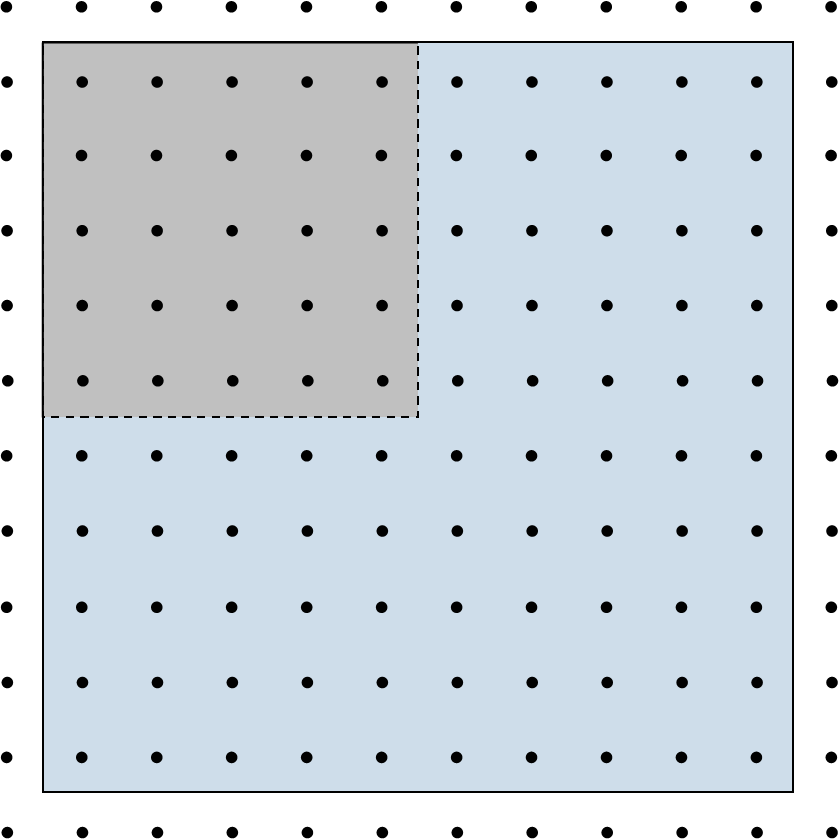
\includegraphics[width=0.5\linewidth]{2d_unit_cell_1.png}
		\caption[The heterogeneous 2D unit cell]{A single 2D unit cell forms the building block of the 2D model. An example lattice arrangement is overlayed on the model to show possible particle positions. The dimensions of each domain can be adjusted individually by changing the number of lattice sites used to define each dimension. Dashed lines represent semi-permeable boundaries and lattice sites (dots) outside the cell belong to adjacent cells.}
		\label{fig:2d_unit_cell_1.png}
	\end{figure}

	%Fixed step-sizes lead to lattice-like arrangement of particle positions. 
	\newpage
	It was decided from the start of the project that particles would move in the system by a constant jump/step-size, compared to a continuum step-size (ex. Gaussian). Although this particle behaviour is generally less representative of a real diffusion process and less accurate compared to continuum Monte Carlo (MC) methods and molecular dynamics simulations, the data generated would still be sufficiently accurate for our analytical purposes and be faster to compute. Fixed step-sizes in the particle movement results in a grid or lattice-like arrangement of particle positions over time. The process simulated is therefore said to be occur on a lattice as the particles are free to move, but only to fixed lattice positions. This manner of particle movement was implemented in both the MC and master equation (ME) simulations.

	%Wrap up, cover remaining details, and state general goals of the simulations. 
	Overall, the goals were to simulate the process of diffusion for homogenous and heterogeneous systems using MC and ME methods, calculate a mean-square-displacement (MSD) for every time step from the computed density distribution, and from the MSD, determine an effective diffusivity and `beta-factor' for the system at any point in time. For both the MC and ME simulations, the particle density distribution data output was of the same form. MSD calculation implementations varied slightly between the MC and ME simulations, but the calculations for effective diffusivity were the same. 	

%Further arrangement possibilities; do we sort the simulations by MC and ME sections with subsections on 1D and 2D systems with further subsubsections on homogenous and heterogenous systems? Even if we sort by 1D and 2D sections with homogenous and heterogenous subsections we still need to divide MC and ME into subsubsections. Too much nesting, I want to go no deeper than 2 nest levels and I don't want to have too much information in a single section and have a few lines in a subsection, it doesn't look good.

\section{Monte Carlo Simulations}
\label{section:mc-sims}
%General structure notes: should not really cover the theory of Monte Carlo, rather the implementation and related details. Introduction applicable to all systems, why Monte Carlo, general pseudo-code example.

	Using MC-based algorithms, information on the individual state of each particle including current position and path history, can be maintained. However, due to the finite number of particles used in the simulation and the stochastic nature of individual particle motion, statistical fluctuations lead to `non-smooth' density distributions. The use of MC algorithms in simulating the process of diffusion was motivated by the random nature of the diffusion process at the level of the individual particle.

\subsection{1D Homogenous and Heterogeneous Systems}
\label{section:mc-sims-1D}
	A natural starting point for the project was 1D systems since they are more simple to model and simulate/program than those which are multidimensional. In our 1D simulations, particles move along a line and at any given lattice site, can move to either one of the two neighbour sites, unless an absolute boundary is met. A particle step-size of one lattice unit was used, meaning that a particle stepped only a single lattice site in a randomly selected direction, each time step. This stepping distance is currently uncorrelated/uncalibrated with any physical or real distance. Each time step in the simulation is also uncorrelated with any characteristic or real time; in the simulation it is simply an integer used as a loop variable. Length and time-scale correlation with physical systems is possible but such an endeavour is outside the time limits of the current project.
	
	In the homogenous system (Figure \ref{fig:1d_unit_cell_1.png}) where particle motion is unbiased, a particle that is not at the absolute lattice limits has an equal probability to step one lattice unit in either direction (we'll use the $ x $-direction). Let those probabilities be: $ P_x^+ $ and $ P_x^- $. The unbiased particle motion requirement is met by ensuring $ P_x^+ = P_x^- $. We can introduce another physically sensible probability; the probability that a particle does not move in a given time step. Let this probability that a particle stays at its current lattice site for the time step be: $ P_x^s = 1 - P_x^+ - P_x^- $. If not at an absolute boundary, the particle has three possible future states. At the absolute boundaries, the particle has only two possible future states; it may move from its current lattice site in a direction away from the boundary, or it may stay at its current lattice site. For example, with reference to Figure \ref{fig:1d_unit_cell_1.png}, if the particle is at the leftmost boundary, then it can only move to the right neighbour lattice site or stay at its current lattice site. Therefore the probabilities for the particle's motion depend on its position within the system and for this example they are: $ 0 < P_x^+ \leq 1 $ and $ P_x^s = 1 - P_x^+ $. It should be noted that reflecting boundaries in the simulation model a situation where a particle attempts to move through the boundary, but is `reflected' back to its starting position. Therefore, in the simulations, the probability of moving towards the boundary is not zero, it is the probability of crossing the boundary that is zero. Since the events of moving towards the boundary and crossing the boundary are treated as mutually exclusive, the total probability of a particle transition into a different domain is the product of the two individual probabilities. In the simulations, the position of the particle within the system is determined and $ P_x^s $ and $ P_x^{-,+} $ are automatically appropriately set. At this point, it may be interesting to ask ``What if the transition probability is not zero at the absolute boundaries?". If the computer simulation does not break from accessing memory space outside a predefined array, then one obtains the case for a semi-permeable boundary and this will be explained later on.
	
	\begin{figure}[h]
		\centering
		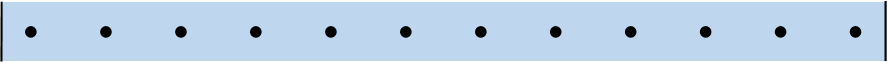
\includegraphics[width=1.0\linewidth]{1d_unit_cell_1.png}
		\caption[Homogenous 1D cell model]{Homogenous 1D cell model with lattice overlay. The sold lines represent the absolute physical limits of the system and behave as reflecting boundaries.}
		\label{fig:1d_unit_cell_1.png}
		\end{figure}	
	
	In the heterogeneous system (Figure \ref{fig:1d_unit_cell_2.png}), a particle that is not at the absolute lattice limits and is not at a lattice site next to a semi-permeable boundary, has an equal probability to step one lattice unit in either direction, the same as in the homogenous system simulation. Particle behaviour at the absolute boundaries was handled the same way as in the homogenous system. The different diffusivities of the cellular and extracellular regions were simulated by using different stepping probabilities. We introduce the subscripts $ i $ and $ e $ to differentiate between stepping probabilities in the (\textsl{intra})cellular and extracellular domains: $ P_{x,i}^{+,-} $ and $ P_{x,e}^{+,-} $. Within each domain and excluding the lattice points at the boundaries, the behaviour of the particles was like that of the homogenous system. At the semi-permeable boundaries, the following condition (Section \ref{sec:intro-diffusion}, ``Detailed Balance") was necessary if the long-time density distribution was to be physically reasonable:
	
	\begin{equation}
		\label{eq:isothermal}
		P_{\textrm{e}\rightarrow \textrm{i}} = \left( \dfrac{P_{x,\textrm{i}}}{P_{x,\textrm{e}}}\right)  P_{\textrm{i}\rightarrow \textrm{e}}
	\end{equation}
	
	This equation relates the boundary transition probabilities $ P_{\textrm{e} \rightarrow \textrm{i}} $ (extracellular to cellular transition) and $ P_{\textrm{i} \rightarrow \textrm{e}} $ (cellular to extracellular transition) between regions of different diffusivities, characterized by the directional stepping probabilities $ P_{x,\textrm{i}} $ and $ P_{x,\textrm{e}} $, \emph{under the condition} $ P_{x,\textrm{i}} < P_{x,\textrm{e}} $ (Section \ref{sec:intro-diffusion}). Note that $ P_{\textrm{e} \rightarrow \textrm{i}} $ \textsl{or} $ P_{\textrm{i} \rightarrow \textrm{e}} $ may be set arbitrarily, but one determines the other according to Equation \ref{eq:isothermal}; they cannot be set independently if the correct density distribution in the long time is desired. 
	
	As an example, consider a particle at a lattice site adjacent to semi-permeable boundary. If the particle is in a cellular region, the total transition probability for the particle to the extracellular region is the product of the transition probability from the cellular to extracellular region and the \textsl{cellular} directional stepping probability.
	
	\begin{equation}
		\label{eq:total_transition_prob}
		P_{\textrm{total},\, \textrm{i} \rightarrow \textrm{e}} = \left( \dfrac{P_{x,\textrm{e}}}{P_{x,\textrm{i}}}\right)  P_{\textrm{e}\rightarrow \textrm{i}} \cdot P_{x,\textrm{i}}
	\end{equation}
	
	Using Equation \ref{eq:isothermal} for the transition probabilities, the total transition probability across any semi-permeable boundary can be determined. In the case of absolute reflecting boundaries, the transition probabilities in Equation \ref{eq:isothermal} are zero, and hence the total transition probability is zero.
	
	\begin{figure}[h]
		\centering
		
\includegraphics[width=1.0\linewidth]{1d_unit_cell_2.png}
		\caption[Heterogeneous 1D cell model]{Heterogeneous 1D unit cells with cellular and extracellular regions. Dashed lines indicate semi-permeable boundary, separating regions characterized by different diffusivities. Dots outside coloured regions indicate continuity of system.}
		\label{fig:1d_unit_cell_2.png}
	\end{figure}
	
	\newpage
	All directional stepping probabilities, boundary transition probabilities, region dimensions, number of particles used, and time step limit are initialized prior to running the simulation. More specifically, the region dimensions are defined by a number of lattice sites used for that region (i.e. the length of a cellular space could be set as $ n $ lattice sites) and the size of a unit cell is the sum of lattice sites in the cellular and extracellular regions. Therefore, the density of lattice sites within any region is always the same, regardless of the size of that region. The total length of the system is the product between the number of lattice sites used in a unit cell and the number of unit cells.
	 	
	Our MC-based simulations of diffusion require a `random' number generator. Pseudo-random numbers, drawn from a uniform distribution, were generated during the execution of the simulation using the \texttt{rand()} C-library function and \texttt{RAND\textunderscore MAX} built-in constant. It was desired that the random numbers ($ rnd $) be uniformly distributed over the interval $ 0 \leq rnd < 1 $, so all random numbers returned by the \texttt{rand()} call were normalized by \texttt{RAND\textunderscore MAX}.
	
	The simulations produced a particle density distribution at every time step. One of the goals of this project was to compute the MSD of the particles at every time step and collect this data for further analysis. Since the individual position of each particle was tracked during the simulation, it was possible to calculate the MSD of all particles for a time $ t_n $. Let $ x_i $ be the position of the $ \textrm{i}^\textrm{th} $ particle at $ t_n $, the MSD is:
	
	\begin{equation}
		\langle \Delta x^2 \rangle = \langle x_{i}^2 \rangle + \langle x_i \rangle^2
	\end{equation}
	
	The angle brackets indicates the sum of the positions divided by the number of particles:
	
	\begin{equation}
		\langle x_{i}^2 \rangle = \dfrac{1}{N}\sum_{i=1}^{N} x_{i}^2
	\end{equation}
	
	\begin{equation}
		\langle x_{i} \rangle = \dfrac{1}{N}\sum_{i=1}^{N} x_i
	\end{equation}
	
	Since the particles experienced no external force, it was expected and shown that for every time step, $ \langle x_{i} \rangle \approx x_0 $, where $ x_0 $ is the position/index of the initial starting lattice site of all the particles. The mean-squared-position $ \langle x_{i}^2 \rangle $ was not constant for every time step, it increased with time reflecting the `spreading' of the particles outwards from their origin.
	
%	The effective diffusivity of the system is obtained in long-time limit using the Einstein-Smoluchowsky relation (kinetic theory):
%	The diffusivity (diffusion coefficient) of the system at any point in time can be obtain using the relation (Section \ref{sec:intro-diffusion}).
%	
%	\begin{equation}
%		D = \frac{\langle \Delta x^2 \rangle}{d\cdot t}
%	\end{equation}
%	
%	where $ d $ is the dimensionality of the system, 1 for 1D systems and 2 for 2D systems.
%	
%	CONTINUE HERE
%	
%	\hrulefill
	
	The output of our simulations was two *.txt files. One file contained the density distribution data computed at every time step. The second file contained the simulation analytics: $ \langle x_{i} \rangle $, $ \langle x_{i}^2 \rangle $, and MSD data computed from the density distribution for every time step. These quantities were all that was needed for further calculations and the creation of various plots for analysis purposes. From the MSD, effective particle diffusivities and the `beta factor' could be computed for various cellular and extracellular diffusivities, semi-permeable boundary transition probabilities, and geometrical variations of the model. The density distribution data was processed by a separate program to create plots for every time step; the result an animation of the particle diffusion process in the system.
	
\subsection{2D Heterogeneous Systems}
\label{section:mc-sims-2D}
	Simulations of particle diffusion were also performed for 2D systems. The 2D model developed and simulated was heterogeneous; no homogenous model was developed. The MC algorithm for the simulation of the 2D system was in principle the same as for the 1D heterogeneous system, however, there are a few important differences to note. For every given time step, a particle at some lattice site that is not at an absolute boundary has four directional steps available and particle movement in the orthogonal directions are independent but cannot both occur in a single time step. Similar  to the 1D simulation, the 2D unit cell is the building block of the 2D model, the particle moves `on a lattice', and a step-size of one lattice unit is permitted. Each unit cell consists a cellular region separated from an extracellular region by a semi-permeable boundary. A key characteristic of the unit cell is that, when linked in series, an extracellular channel is formed providing particles the option to move freely without obstruction. In Figure \ref{fig:2d_unit_cell_2.png}, this is visible as an uninterrupted region or channel in the lower half of the figure. It is possible to arrange more than one series of unit cells so that a larger $\left(  m \times n \right) $ unit cell configuration is obtained, but this was not studied. Only $\left(  1 \times n \right) $ unit cell models were simulated. 
	
	\begin{figure}[h]
		\centering
		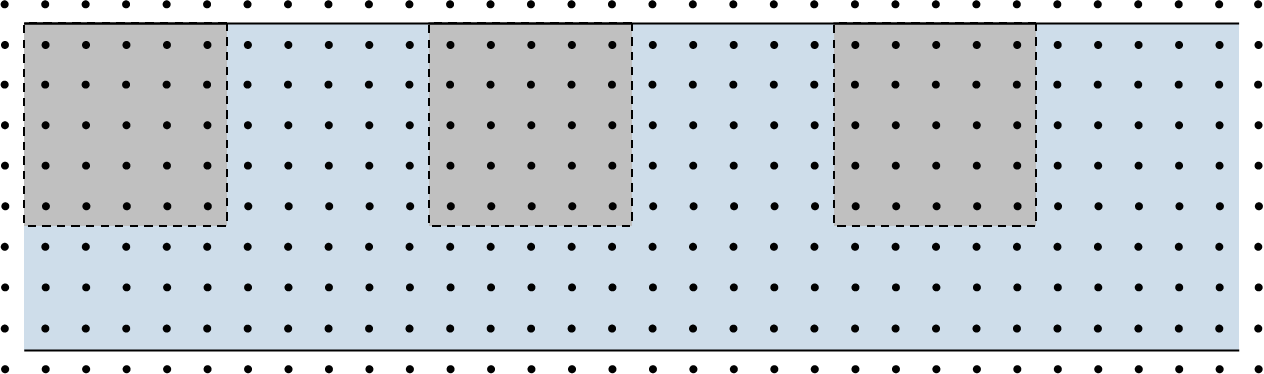
\includegraphics[width=1.0\linewidth]{2d_unit_cell_2.png}
		\caption[Series configuration of heterogeneous 2D unit cells]{A $ \left( 1 \times n \right) $ series configuration of 2D unit cells with cellular and extracellular regions. Dashed lines indicate semi-permeable boundary and solid lines indicate absolute boundary. Dots outside the coloured region indicate continuity of the system.}
		\label{fig:2d_unit_cell_2.png}
	\end{figure}
	
	In 2D, there are an additional two neighbour lattice sites the particle can move to. If not at an absolute boundary, the particle has five possible future states. At the absolute boundaries, the particle has only 4 possible future states; it may move from its current lattice site in a direction away from the boundary, along the boundary, or it may stay at its current lattice site. We introduce an additional set of directional stepping probabilities in $ \hat{y} $: $ P_{y,i}^{+,-} $ and $ P_{y,e}^{+,-} $. The directional stepping probabilities in $ \hat{x} $ and $ \hat{y} $ have the conditions: $ 0 < P_{i,e}^{+,-} \leq 0.25 $. For unbiased motion (excluding boundary lattice sites) all directional stepping probabilities must be equal. Therefore, the probability that the particle y-coordinate does not change for a given time step is $ P_{y}^s = 1 - P_{y}^{+} - P_{y}^{-}$. Similarly for the x-coordinate $ P_{x}^s = 1 - P_{x}^{+} - P_{x}^{-}$. So the total probability that a particle remains at its current lattice site is $ P^s = 1 - P_{x}^s - P_{y}^s$. When a random number is generated, its value is tested for membership in intervals defined by the stepping probabilities, and this determines the motion of the particle.
	
	Handling of the boundary transition probabilities was done in the same manner as the 1D simulation, in accordance with Equation \ref{eq:isothermal}. In the program developed, for every time step, the current particle position and possible future particle position are compared. If it is found that the future possible position is in a different region than the current position, then the probability to cross into the new region is automatically set using Equation \ref{eq:total_transition_prob} solved for $ P_{\textrm{total},\, \textrm{i} \rightarrow \textrm{e}} $ or $ P_{\textrm{total},\, \textrm{e} \rightarrow \textrm{i}} $. Absolute boundaries were implemented as reflecting boundaries.
	
	Similar to the 1D simulations, density distribution data and other analytical data was computed and written to *.txt files. The density distribution data output was in a matrix form; each line of data represented a different row of lattice sites in the system. For each time step, all rows were written to the file and an empty line inserted before writing data for the next time step, for parsing purposes. Producing 2D animations of the diffusion process required a program different than the one used to create the 1D animations; however, similar programs were used to simulation analytics.

\section{Master Equation Simulations}
\label{section:me-sims}
%General structure notes: should not really cover the theory of master equations, rather the implementation and related details. A, B, general pseudo-code example. An issue here might be figures; the same general figures are used in both sections... so where should they be presented?
	
	Using the ME methods and evolving the particle density distribution in time, discontinuities in the distributions due to statistical fluctuations are no longer an issue; however, at the expense of information on individual particle state. Using this method, it is not possible to know individual particle position history which restricts the use of certain analyses. For example, it is not possible to reconstruct the paths of particles through the system which can be used to generate a frequency histogram to score the number of times a particle crosses a semi-permeable boundary. The main reason for use of the ME methods was that most of our intended analysis only required knowledge of $ \langle x_{i} \rangle $, $ \langle x_{i}^2 \rangle $, and MSD. These quantities could be calculated, although in a slightly different way than implemented in the MC methods. In addition, for the basic models simulated, ME-based simulations were much faster than MC-based simulations. ME simulations were also performed on a lattice and within cellular or extracellular regions, directional stepping probabilities were equal for unbiased motion.
	
	Consider the situation of a single particle at a lattice site that, at a given time step, has a directional stepping probability of $ P_x^{+,-} = 0.5 $ (similar to a coin-toss experiment). In the MC simulations, a random number is drawn from uniform distribution and tested for membership in the intervals defined by the directional stepping probabilities.
	
	\[   \left\{
	\begin{array}{ll}
	      x_0 - 1 & P_x^{-}: 0.0 \leq \textrm{rnd} < 0.5 \\
	      x_0 + 1 & P_x^{+}: 0.5 \leq \textrm{rnd} < 1.0 \\
	\end{array} 
	\right. \]
	
	For a small, even number $ N $ of particles, it may not be reasonable to expect that the number of particles that step $ -1 $ or $ +1 $ in $ \hat{x} $ is exactly N/2. In terms of particle positions, even though the particles have an equal probability of stepping in either direction, the mean position of the particles $ \langle x \rangle $ will likely not equal $ x_0 $, the expected value of the mean position. However, the law of large numbers guarantees that the arithmetic mean of the position of the particles practically converges to the expected value in the limit of very many particles. In the ME simulations, it is assumed that there are very many particles, enough that the fluctuation in the mean position of the particles is also assumed zero. Instead of starting with some number of particles at $ x_0 $, we start with a particle density $ \rho_0 $ at $ x_0 $ and evolve the particle density distribution in time. % As an example, if the density is $ \rho(x_0) = \rho_0 $ with the stepping probabilities $ P_x^{+,-} = 0.2 $ and $ P_x^{s} = 0.6 $, then at the next time we have the density distribution $ \rho(x_0 - 1) = \rho(x_0 + 1) = 0.2 $ and $ \rho(x_0) = 0.6 $. 
	
	At absolute and semi-permeable boundaries, the density distribution was, in principle, treated similar to how individual particles were treated in MC. Instead of the value of a random number determining the movement of a particle, the evolution of the density distribution to the next time step depended on the probability distribution of possible particle movements at that lattice site. Clarifying with an example, consider a lattice site with particle density $ \rho_0 $ in a cellular region and adjacent ($ -\hat{x} $) to the site is a semi-permeable boundary. The boundary transition probability follows Equation \ref{eq:isothermal} solved for $ P_{\textrm{i} \rightarrow \textrm{e}} $ and the total transition is probability is:
	
	\begin{equation}
		P_{\textrm{total},\, \textrm{i} \rightarrow \textrm{e}} = \left( \dfrac{P_{x,\textrm{e}}}{P_{x,\textrm{i}}}\right)  P_{\textrm{e}\rightarrow \textrm{i}} \cdot P_{x,\textrm{i}}
	\end{equation}	
	
	Therefore, the density distribution at the next time step is:
	
	\[   \left\{
	\begin{array}{l}
	      \rho(x_0 - 1) =   \rho_0(x_0) \cdot P_{\textrm{total},\, \textrm{i} \rightarrow \textrm{e}} \\
	      \rho(x_0 + 1) =   \rho_0(x_0) \cdot P_{x,\textrm{i}} \\
	      \rho(x_0) =   1 - \rho_0(x_0) \cdot P_{\textrm{total},\, \textrm{i} \rightarrow \textrm{e}} -  \rho_0(x_0) \cdot P_{x,\textrm{i}}\\
	\end{array} 
	\right. \]	
	
	This time-evolution of the density distribution was essentially performed by looping over all lattice sites each time step and at a given lattice site, applying the appropriate directional probabilities (product with the particle density at the corresponding site). 
	
	%An array of values was created; each element of the array corresponded to a lattice site and had a unique value depending on its location in the model, cellular or extracellular region. Next, a set of commensurate `directional probability' arrays was created. Each array 
	
	As previously mentioned, the quantities $ \langle x_{i} \rangle $, $ \langle x_{i}^2 \rangle $, and MSD were calculated slightly differently than in the MC simulations, since the position of an individual particle was not known. Known was the density $ \rho_i $ at each lattice site  $ i $. If the starting density was initialized as $ \rho_0 = 1.0 $, then at any time step:
	
	\begin{equation}
		\langle x_{i}^2 \rangle = \sum_{i=1}^{N} i \cdot \rho_i 
	\end{equation}
	
	\begin{equation}
		\langle x_{i} \rangle = \sum_{i=1}^{N} i^2\cdot \rho_i
	\end{equation}
	
	The same programs that were used to create the diffusion process animations and other plots for the 1D and 2D MC simulations, were used for the ME simulations since the output data was the same. Most of the analyses of 2D diffusion were based on ME simulations since the MC simulations took too much time to test various parameter combinations. At least 1 million time steps were needed to observe various diffusive regimes on an `infinite' in $ \hat{x} $ system ($ 30 \times 3330$ grid of lattice points was usually enough).
	
	%Application of both methods to calculate the effective particle diffusivities and to determine density distribution profiles. What kind of agreement do we have between the results from the two different methods? Both methods involve discretization (of what?) and so there is always some amount of discretization error. Is it negligible for our modelling purposes?
	
